
\chapter{Конструкторская часть}
В данной части работы будет описана реализация базы данных, описана ER диаграмма БД и принципиальная схема БД, также будут описаны схемы триггеров и хранимые процедуры.


\section{Формализация взаимодействия с приложением}


Системе автоматической проверки необходимо проверить на правильность составные части отчета, что подразумевает детекцию рисунков, графиков, схем алгоритмов, списка используемых источников, а также формул.

На рисунках \ref{img:detection}--\ref{img:detection_inside} представлены результаты разработки системы детекции составных частей.

\includeimage
{detection} % Имя файла без расширения (файл должен быть расположен в директории inc/img/)
{f} % Обтекание (без обтекания)
{H} % Положение рисунка (см. figure из пакета float)
{1\textwidth} % Ширина рисунка
{IDEF0 обнаружение составных частей отчет 0 уровня} % Подпись рисунка

\includeimage
{detection_inside} % Имя файла без расширения (файл должен быть расположен в директории inc/img/)
{f} % Обтекание (без обтекания)
{H} % Положение рисунка (см. figure из пакета float)
{1\textwidth} % Ширина рисунка
{IDEF0 обнаружение составных частей отчета 1 уровня} % Подпись рисунка

После решения задачи детекции необходимо проверить составные части на соответствие ГОСТ 7.32, однако, финальный вердикт должен выноситься экспертом. На рисунках \ref{img:errors}--\ref{img:errors_inside} представлены результаты разработки данной системы.

\includeimage
{errors} % Имя файла без расширения (файл должен быть расположен в директории inc/img/)
{f} % Обтекание (без обтекания)
{H} % Положение рисунка (см. figure из пакета float)
{1\textwidth} % Ширина рисунка
{IDEF0 проверки составных частей отчета на соответствие ГОСТ 7.32 0 уровня} % Подпись рисунка

\includeimage
{errors_inside} % Имя файла без расширения (файл должен быть расположен в директории inc/img/)
{f} % Обтекание (без обтекания)
{H} % Положение рисунка (см. figure из пакета float)
{1\textwidth} % Ширина рисунка
{IDEF0 проверки составных частей отчета на соответствие ГОСТ 7.32 1 уровня} % Подпись рисунка
\newpage
\section{Формализация работы системы проверки отчета}
На рисунке~\ref{img:main_sys_bpmn}, представлена схема BPMN 2.0 работы системы в процессе проверки отчета, а также всех взаимодействующих с ней акторов.
\begin{sidewaysfigure}[H]
	\centering
	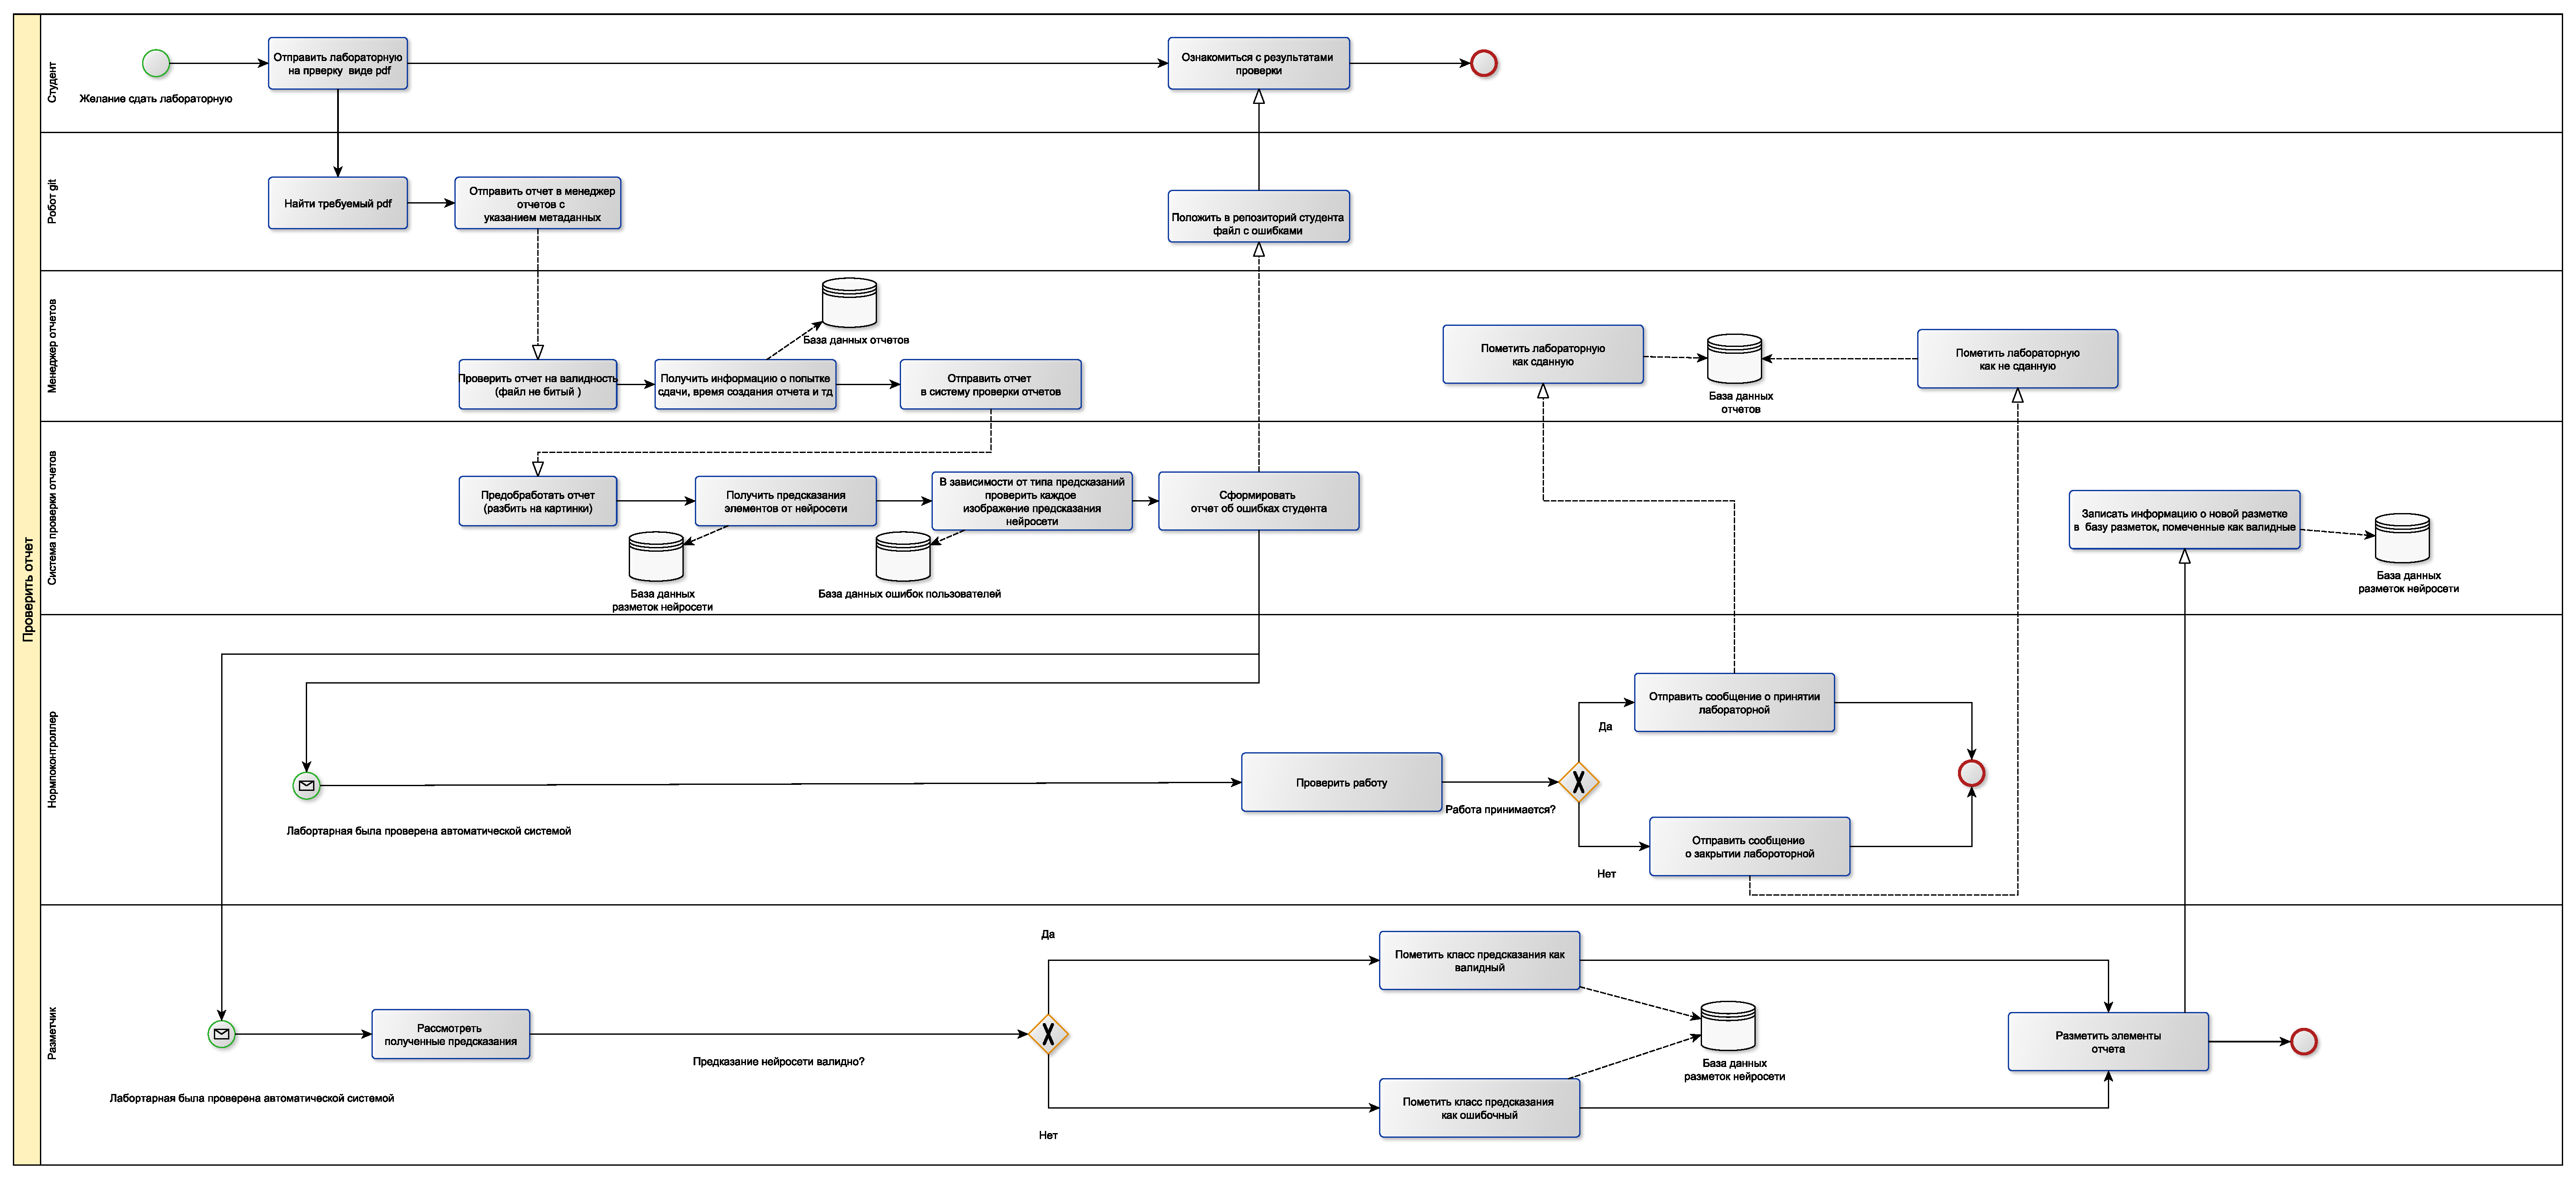
\includegraphics[width=\textwidth]{./inc/img/process_check_bpmn.pdf}
	\caption{Схема BPMN 2.0 работы системы}
	\label{img:main_sys_bpmn}
\end{sidewaysfigure}


\section{Формализация сущностей базы данных}

В соответствие с диаграммами~\ref{img:errors}--\ref{img:errors_inside} были выделены следующие таблицы:
\begin{enumerate}
	\item студент --- сущность студента (имеет уникальный идентификатор для связи со сданными отчетами и комментариями);
	\item нормоконтроллеер --- сущность нормоконтроллера (имеет уникальный идентификатор для связи с проверенными отчетами и созданными ошибками);
	\item выделенный фрагмент --- сущность ошибок в отчетах студентов (хранит страницу отчета с ошибкой, а также данные, указывающие на местоположение ошибки, а также тип фрагмента);
	\item тип фрагмента~---~сущность типов ошибок (необходима для введения новых типов ошибок, хранит описание ошибки);
	\item отчет --- сущность отчета студента (хранит все страницы попытки сдачи отчета, а также время сдачи и номер попытки сдачи);
	\item комментарий --- сущность комментария студента о ошибке (в случае ошибки преподавателя можно указать на это, кроме данных комментария хранит идентификатор студента, создавшего комментарий);
	\item достижение --- сущность награды для выдачи студентам, преуспевающим в выполнении лабораторных работ (хранит идентификатор студента, которому выдали награду, а также идентификатор отчета, за который было получено достижение).
\end{enumerate}

\section{Ограничения целостности базы данных}
В данной части работы будут описаны описаны поля сущностей баз данных и их ограничения, для обеспечения целостности данных системы. Ограничение <<первичный ключ>> подразумевает то что поле сущности является первичным ключом данного отношения в реляционной модели данных.
\begin{table}[h!tbp]
	\centering
	\caption{Ограничение целостности сущности отчета}
	\begin{tabularx}{\textwidth}{|X|X|X|}
		\hline
		Поле & Тип & Ограничение \\
		\hline
		id & целое число & первичный ключ \\
		\hline
		page\_count & целое число & не пустое значение\\
		\hline
		document\_name & строка & не пустое значение\\
		\hline
		checks\_count & целое число & не пустое значение\\
		\hline
		creator\_id & целое число & не пустое значение\\
		\hline
		creation\_time & дата и время & не пустое значение\\
		\hline
	\end{tabularx}

	\label{t:documents_cons}
\end{table}

\begin{table}[h!tbp]
	\centering
	\caption{Ограничение целостности сущности фрагмента}
	\begin{tabularx}{\textwidth}{|X|X|X|}
		\hline
		Поле & Тип & Ограничение \\
		\hline
	  	id & целое число & первичный ключ \\
	  	\hline
		description & строка & не пустое значение \\
		\hline
		creator\_id & целое число & не пустое значение\\
		\hline
		class\_name & строка & не пустое значение\\
		\hline
	\end{tabularx}
	
	\label{t:markup_type_cons}
\end{table}

\begin{table}[H]
	 \centering
	 \caption{Ограничение целостности сущности типа фрагмента}
	\begin{tabularx}{\textwidth}{|X|X|X|}
		\hline
		Поле & Тип & Ограничение \\
		\hline
		id & целое число & первичный ключ \\
		\hline
		page\_data & байты изображения & не пустое значение\\
		\hline
		error\_bb & массив из 4 вещественных чисел & не пустое значение\\
		\hline
		class\_label & целое число & не пустое значение\\
		\hline
		creator\_id & целое число & не пустое значение\\
		\hline
	\end{tabularx}
	\label{t:markups}
\end{table}




\begin{table}[h!tbp]
	\centering
	\caption{Ограничение целостности сущности пользователя}
	\begin{tabularx}{\textwidth}{|X|X|X|}
	\hline
	Поле & Тип & Ограничение \\
	\hline
	id & целое число & первичный ключ\\
	\hline
	login & строка & уникальный,не пустое значение\\
	\hline
	password & строка & не пустое значение\\
	\hline
	name & строка & не пустое значение\\
	\hline
	surname & строка & не пустое значение\\
	\hline
	role\_id & целое число & не пустое значение\\
	\hline
	role\_type & строка & не пустое значение\\
	\hline
	group & строка & не пустое значение\\
	\hline
	\end{tabularx}
	\label{t:users_cons}
\end{table}


\begin{table}[h!tbp]
	\centering
	\caption{Ограничение целостности сущности достижения}
	\begin{tabularx}{\textwidth}{|X|X|X|}
		\hline
		Поле & Тип & Ограничение \\
		\hline
		id & целое число & первичный ключ\\
		\hline
		picture & байты изображения &  не пустое значение\\
		\hline
		text & строка & не пустое значение\\
		\hline
		creator\_id & целое число & не пустое значение\\
		\hline
		granted\_to\_id & целое число & не пустое значение \\
		\hline
	\end{tabularx}
	\label{t:achievment_cons}
\end{table}

\begin{table}[h!tbp]
	\centering
	\caption{Ограничение целостности сущности комментария}
	\begin{tabularx}{\textwidth}{|X|X|X|}
		\hline
		Поле & Тип & Ограничение \\
		\hline
		id & целое число & первичный ключ\\
		\hline
		description & строка & не пустое значение\\
		\hline
		creator\_id & целое число & не пустое значение\\
		\hline
		report\_id & целое число & не пустое значение\\
		\hline
	\end{tabularx}
	\label{t:comment_cons}
\end{table}






\section{Ролевая модель}
Была определена следующая ролевая модель:
\begin{enumerate}
	\item Разметчик --- имеет права доступа SELECT к таблице документов и INSERT к таблице выделенных фрагментов.
	\item Добавляющий --- имеет права доступа INSERT к таблице студентов и нормоконтроллеров
	\item Пользователь --- имеет права доступа INSERT к таблице комментариев, имеет права доступа SELECT  и INSERT к таблице выделенных фрагментов.
	\item Нормоконтроллер --- является разметчиков, также имеет права доступа INSERT и SELECT к таблице тип\_ошибки и таблице достижений.
	\item Администратор имеет все права доступа ко всем таблицам.
	\item Также выделяется работник очереди задача которого --- работать с отчетами из очереди и помечать их как проверенные,имеет права доступа SELECT и UPDATE к очереди документов.
	\item При проверке документов из очереди система работает в роли работника очереди, в иных случаях система использует роль администратора.
\end{enumerate}

\section{Определение модели базы данных}
Необходимо определить модель базы данных, которая будет использована для хранения информации в системе. Реляционная модель баз данных позволяет хранить сущности в целостном виде и поддерживает сложные запросы, поэтому она является наилучшим выбором для поставленной задачи. Также необходимо хранить файлы журнала приложения, ввиду частого его пополнения и необходимости частой записи стоит использовать базу данных временных рядов.

\section{Используемые триггеры}
В базе данных присутствует триггер, запускающий процесс обнаружения ошибок в отчете при добавлении отчета в базу данных. При вставке экземпляра отчета в базу данных, в случае, если данный отчет не был до этого проверен и не имеет в имени файла VIP (такие файлы обслуживаются вне очереди), он будет добавлен в очередь отчетов. Очередь отчетов представляет собой таблицу, в который хранится ID отчета и его статус (не обработан, обработан, обработан с ошибкой).
\includeimage
{add_queue_trigger} % Имя файла без расширения (файл должен быть расположен в директории inc/img/)
{f} % Обтекание (без обтекания)
{H} % Положение рисунка (см. figure из пакета float)
{1\textwidth} % Ширина рисунка
{Схема алгоритма триггера после добавления в таблицу метаданных отчетов} % Подпись рисунка







\section*{Вывод}
В данной части были формализованы процессы автоматической проверки, а также выделены различные виды пользователей: нормоконоктроллер, студент, система и администратор, после чего были определены права для каждого из пользователей.




